\documentclass[aspectratio=169]{beamer}

% ---------- PREAMBLE ----------
\usepackage{array,booktabs}
\usepackage[table]{xcolor}   % rowcolors + colors in tables
\usepackage{colortbl}        % \arrayrulecolor
\usepackage{tikz}
\usetikzlibrary{arrows.meta,positioning,shadows.blur,fit,calc}

% Colors (define once)
\definecolor{pri}{RGB}{0,120,212}   % primary blue
\definecolor{acc}{RGB}{3,166,120}   % accent green
\definecolor{mut}{RGB}{120,120,120} % muted gray

% Beamer theme tweaks
\setbeamertemplate{navigation symbols}{}
\setbeamercolor{title}{fg=pri}
\setbeamercolor{frametitle}{fg=pri}
\setbeamerfont{frametitle}{series=\bfseries}

% --- TikZ styles ---
\tikzset{
  router/.style={circle,draw=black,fill=white,very thick,minimum size=9mm,drop shadow},
  link/.style={-Latex,ultra thick,draw=pri!80},  % thicker, blue-toned
  linkmut/.style={-Latex,thick,draw=mut},
  linkdash/.style={-Latex,ultra thick,dashed,draw=acc},
  badge/.style={rectangle,rounded corners=2pt,fill=pri!10,draw=pri,inner sep=2pt,font=\scriptsize},
  % Your upgraded flowstep style (with subtle gradient + shadow)
  flowstep/.style={
    rectangle,rounded corners=4pt,
    draw=black,very thick,
    top color=white,bottom color=pri!5,
    minimum height=8mm,inner sep=6pt, % a bit more padding
    drop shadow
  },
  good/.style={circle,draw=acc,very thick,minimum size=5mm},
  bad/.style={circle,draw=pri,very thick,minimum size=5mm},
}

\title{Static vs Floating Static vs RIP}

% ---------- DOCUMENT ----------
\begin{document}

% ------------------- Slide 1 -------------------
\begin{frame}{Static vs Floating Static vs RIP}
\small

\begin{table}
\centering
\rowcolors{2}{pri!10}{white}
\arrayrulecolor{pri!60}
\begin{tabular}{@{}>{\bfseries\arraybackslash}m{3.2cm}
                >{\centering\arraybackslash}m{3.0cm}
                >{\centering\arraybackslash}m{3.0cm}
                >{\centering\arraybackslash}m{4.2cm}@{}}
\toprule
\rowcolor{pri!25}\bfseries Type & \bfseries Reliability & \bfseries Ease of Setup & \bfseries Ethical Considerations \\
\midrule
Static & High (manual) & Easy (small nets) & Keep routes updated; avoid stale paths \\
\textbf{Floating Static} & High (with backup) & Moderate (priorities) & Don’t abuse metrics to prefer unfair paths \\
\textbf{RIP (Dynamic)} & Adaptive (changes) & Simple, scalable & Secure updates; prevent false adverts \\
\bottomrule
\end{tabular}
\rowcolors{2}{white}{white}
\end{table}

\vspace{0.6cm}
\centering
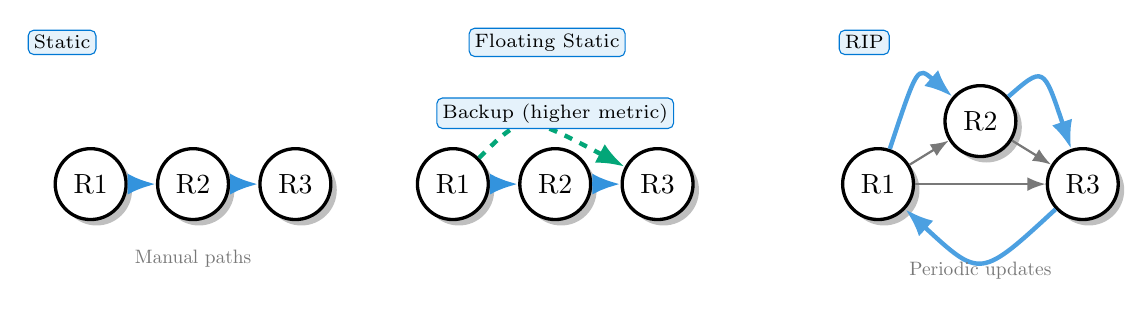
\begin{tikzpicture}[scale=1, every node/.style={transform shape}]
% Labels
\node[badge,anchor=west] (b1) at (-5.8,1.8) {Static};
\node[badge,anchor=west] (b2) at (-0.2,1.8) {Floating Static};
\node[badge,anchor=west] (b3) at (4.5,1.8) {RIP};

% --- Static cluster ---
\node[router] (S1) at (-5,0){R1};
\node[router] (S2) at (-3.7,0){R2};
\node[router] (S3) at (-2.4,0){R3};
\draw[link] (S1) -- (S2);
\draw[link] (S2) -- (S3);
\node[align=center,mut,scale=0.7] at (-3.7,-0.95) {Manual paths};

% --- Floating Static cluster ---
\node[router] (F1) at (-0.4,0){R1};
\node[router] (F2) at (0.9,0){R2};
\node[router] (F3) at (2.2,0){R3};
\draw[link] (F1) -- (F2);
\draw[link] (F2) -- (F3);
% backup diagonal
\draw[linkdash] (F1) .. controls (0.5,0.9) .. (F3);
\node[badge] at (0.9,0.9) {Backup (higher metric)};

% --- RIP cluster ---
\node[router] (D1) at (5.0,0){R1};
\node[router] (D2) at (6.3,0.8){R2};
\node[router] (D3) at (7.6,0){R3};
\draw[linkmut] (D1) -- (D2);
\draw[linkmut] (D2) -- (D3);
\draw[linkmut] (D1) -- (D3);
% dynamic arrows
\draw[-Latex,ultra thick,draw=pri!70] (D1) .. controls (5.5,1.5) .. (D2);
\draw[-Latex,ultra thick,draw=pri!70] (D2) .. controls (7.1,1.5) .. (D3);
\draw[-Latex,ultra thick,draw=pri!70] (D3) .. controls (6.3,-1.2) .. (D1);
\node[align=center,mut,scale=0.7] at (6.3,-1.1) {Periodic updates};
\end{tikzpicture}
\end{frame}

% ------------------- Slide 2 -------------------
\begin{frame}{Best Practices \& Outage Prevention}
\small
\begin{columns}[T,onlytextwidth]

% Left: flow with subtext anchors
\begin{column}{0.55\textwidth}
\centering
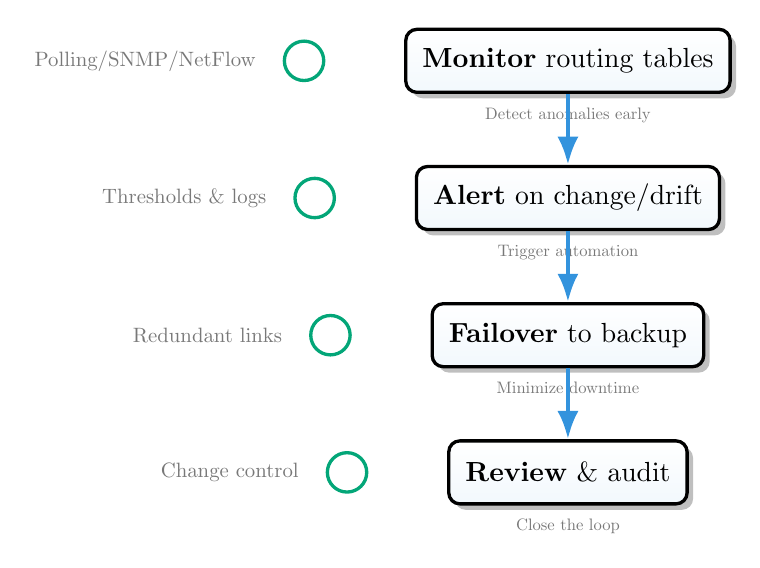
\begin{tikzpicture}[node distance=9mm and 10mm]
\node[flowstep] (m)  {\textbf{Monitor} routing tables};
\node[mut,scale=0.6,below=1mm of m] {Detect anomalies early};

\node[flowstep,below=of m] (a) {\textbf{Alert} on change/drift};
\node[mut,scale=0.6,below=1mm of a] {Trigger automation};

\node[flowstep,below=of a] (f) {\textbf{Failover} to backup};
\node[mut,scale=0.6,below=1mm of f] {Minimize downtime};

\node[flowstep,below=of f] (r) {\textbf{Review} \& audit};
\node[mut,scale=0.6,below=1mm of r] {Close the loop};

% Flow arrows
\draw[link] (m) -- (a);
\draw[link] (a) -- (f);
\draw[link] (f) -- (r);

% side notes (slightly more breathing room)
\node[good,left=10mm of m] (g1) {};
\node[align=right,mut,scale=0.75,anchor=east] at ($(g1.west)+(-0.25,0)$) {Polling/SNMP/NetFlow};

\node[good,left=10mm of a] (g2) {};
\node[align=right,mut,scale=0.75,anchor=east] at ($(g2.west)+(-0.25,0)$) {Thresholds \& logs};

\node[good,left=10mm of f] (g3) {};
\node[align=right,mut,scale=0.75,anchor=east] at ($(g3.west)+(-0.25,0)$) {Redundant links};

\node[good,left=10mm of r] (g4) {};
\node[align=right,mut,scale=0.75,anchor=east] at ($(g4.west)+(-0.25,0)$) {Change control};
\end{tikzpicture}
\end{column}

% Right: topology + concise takeaways
\begin{column}{0.45\textwidth}
\centering
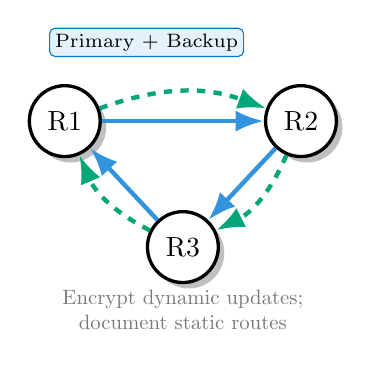
\begin{tikzpicture}
% Redundant mini-topology (primary + backup)
\node[router] (A) at (0,0){R1};
\node[router] (B) at (3,0){R2};
\node[router] (C) at (1.5,-1.6){R3};

\draw[link]    (A) -- (B);
\draw[link]    (B) -- (C);
\draw[link]    (C) -- (A);
% backup links (dashed)
\draw[linkdash] (A) to[bend left=20] (B);
\draw[linkdash] (B) to[bend left=20] (C);
\draw[linkdash] (C) to[bend left=20] (A);

\node[badge,anchor=west] at (-0.2,1.0) {Primary + Backup};
\node[align=center,mut,scale=0.75] at (1.5,-2.4) {Encrypt dynamic updates;\\document static routes};
\end{tikzpicture}

\vspace{2mm}
\footnotesize
\begin{tabular}{@{}>{\bfseries}l l@{}}
Static:   & Update on change \\
Floating: & Test failover \\
RIP:      & Authenticate updates \\
\end{tabular}
\end{column}

\end{columns}
\end{frame}

\end{document}
